\section{実験結果}
実験の結果について述べる.
実験で取得したデータと検定の結果について述べる.

\subsection{回答データ}
\subsubsection{システムグループ}
システムグループの回答について述べる.
鹿児島の旅程に対する災害の深刻さに対する認知と災害発生の確率に対する認知の回答について述べる.
災害の深刻さに対する認知への回答を図 \ref{fig:system_kagoshima_1}に示す.
\begin{figure}[H]
  \centering
  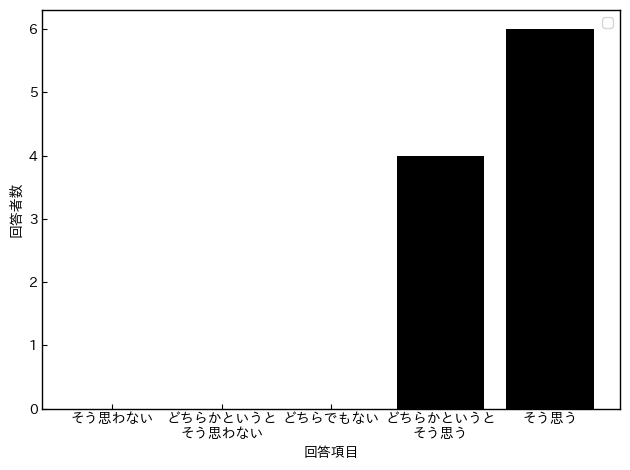
\includegraphics[height=8cm]{./fig/system_kagoshima_1.png}
  %\vspace{-3mm}
  \caption{(鹿児島)旅行中に災害に巻き込まれたとしたら、被害は大きいと思う}
  \label{fig:system_kagoshima_1}
  %\vspace{2mm}
\end{figure}
「そう思わない」と回答した人が0人,「どちらかというとそう思わない」と回答した人が0人,「どちらでもない」と回答した人が0人「どちらかというとそう思う」と回答した人が4人,「そう思う」と回答した人が6人いた.

災害発生の確率に対する認知への回答を図 \ref{fig:system_kagoshima_2}に示す.
\begin{figure}[H]
  \centering
  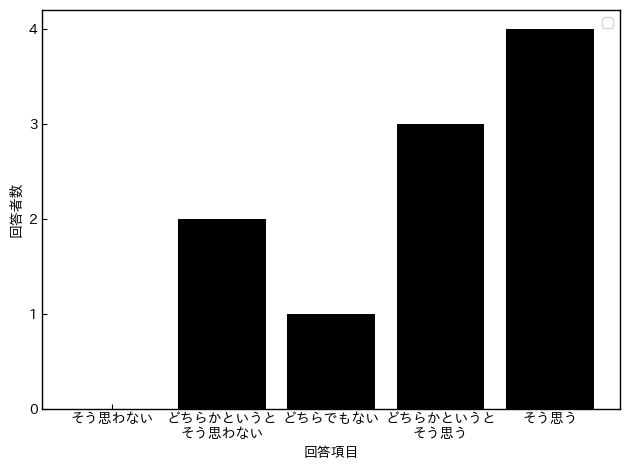
\includegraphics[height=8cm]{./fig/system_kagoshima_2.png}
  %\vspace{-3mm}
  \caption{(鹿児島)旅行中に災害の被害に遭うと思う}
  \label{fig:system_kagoshima_2}
  %\vspace{2mm}
\end{figure}
「そう思わない」と回答した人が0人,「どちらかというとそう思わない」と回答した人が2人,「どちらでもない」と回答した人が1人「どちらかというとそう思う」と回答した人が3人,「そう思う」と回答した人が4人いた.

福岡の旅程に対する災害の深刻さに対する認知と災害発生の確率に対する認知の回答について述べる.
災害の深刻さに対する認知への回答を図 \ref{fig:system_fukuoka_1}に示す.
\begin{figure}[H]
  \centering
  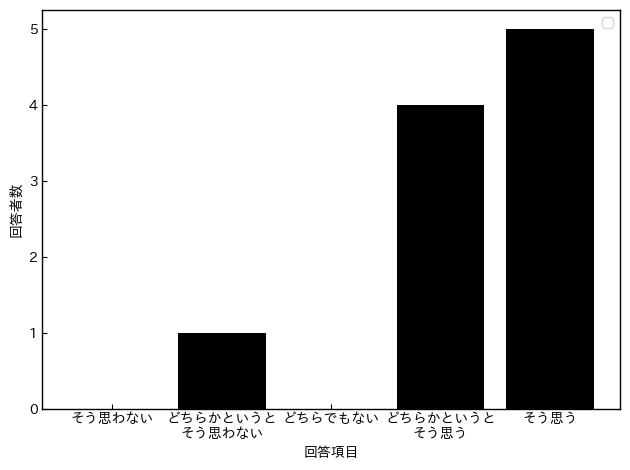
\includegraphics[height=8cm]{./fig/system_fukuoka_1.png}
  %\vspace{-3mm}
  \caption{(福岡)旅行中に災害に巻き込まれたとしたら、被害は大きいと思う}
  \label{fig:system_fukuoka_1}
  %\vspace{2mm}
\end{figure}
「そう思わない」と回答した人が0人,「どちらかというとそう思わない」と回答した人が1人,「どちらでもない」と回答した人が0人「どちらかというとそう思う」と回答した人が4人,「そう思う」と回答した人が5人いた.

災害発生の確率に対する認知への回答を図 \ref{fig:system_fukuoka_2}に示す.
\begin{figure}[H]
  \centering
  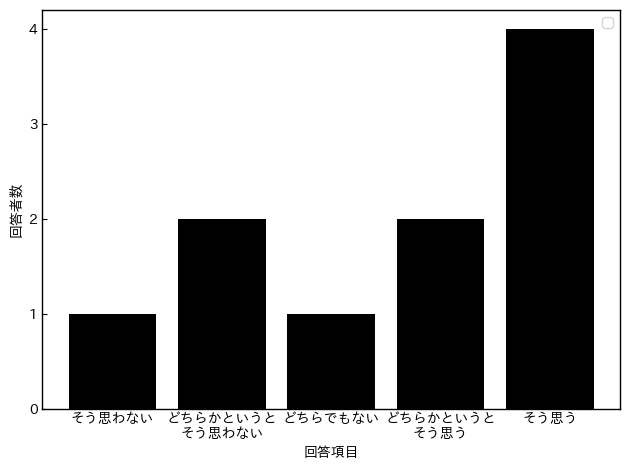
\includegraphics[height=8cm]{./fig/system_fukuoka_2.png}
  %\vspace{-3mm}
  \caption{(福岡)旅行中に災害の被害に遭うと思う}
  \label{fig:system_fukuoka_2}
  %\vspace{2mm}
\end{figure}
「そう思わない」と回答した人が1人,「どちらかというとそう思わない」と回答した人が2人,「どちらでもない」と回答した人が1人「どちらかというとそう思う」と回答した人が2人,「そう思う」と回答した人が4人いた.

\subsubsection{天気予報グループ}
天気予報グループの回答について述べる.

% \subsection{鹿児島の旅程}
鹿児島の旅程に対する災害の深刻さに対する認知と災害発生の確率に対する認知の回答について述べる.
災害の深刻さに対する認知への回答を図 \ref{fig:forecast_kagoshima_1}に示す.
\begin{figure}[H]
  \centering
  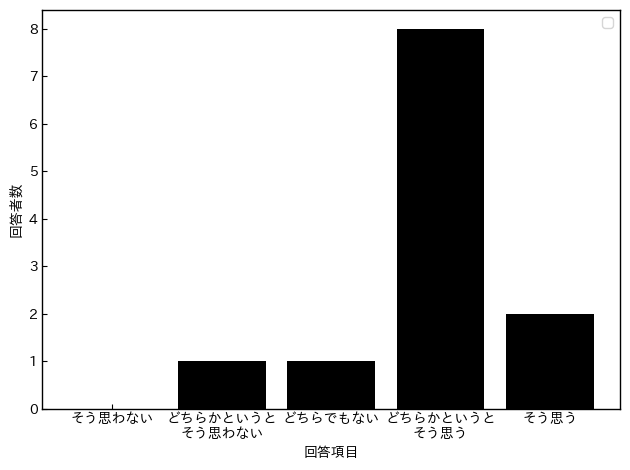
\includegraphics[height=8cm]{./fig/forecast_kagoshima_1.png}
  %\vspace{-3mm}
  \caption{(鹿児島)旅行中に災害に巻き込まれたとしたら、被害は大きいと思う}
  \label{fig:forecast_kagoshima_1}
  %\vspace{2mm}
\end{figure}
「そう思わない」と回答した人が0人,「どちらかというとそう思わない」と回答した人が1人,「どちらでもない」と回答した人が1人「どちらかというとそう思う」と回答した人が8人,「そう思う」と回答した人が2人いた.
災害発生の確率に対する認知への回答を図 \ref{fig:forecast_kagoshima_2}に示す.
\begin{figure}[H]
  \centering
  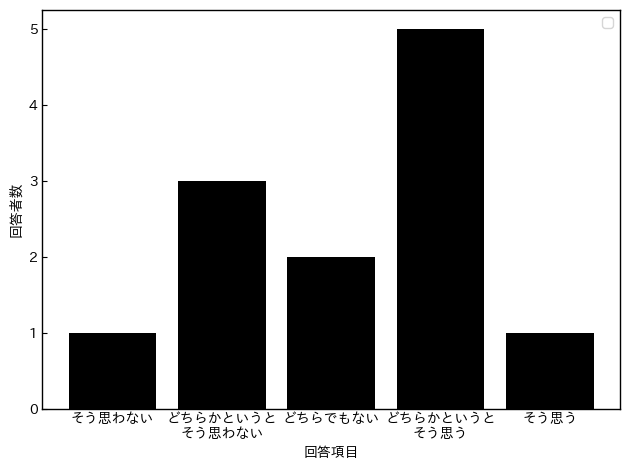
\includegraphics[height=8cm]{./fig/forecast_kagoshima_2.png}
  %\vspace{-3mm}
  \caption{(鹿児島)旅行中に災害の被害に遭うと思う}
  \label{fig:forecast_kagoshima_2}
  %\vspace{2mm}
\end{figure}
「そう思わない」と回答した人が1人,「どちらかというとそう思わない」と回答した人が3人,「どちらでもない」と回答した人が2人「どちらかというとそう思う」と回答した人が5人,「そう思う」と回答した人が1人いた.

% \subsection{福岡の旅程}

福岡の旅程に対する災害の深刻さに対する認知と災害発生の確率に対する認知の回答について述べる.
災害の深刻さに対する認知への回答を図 \ref{fig:forecast_fukuoka_1}に示す.
\begin{figure}[H]
  \centering
  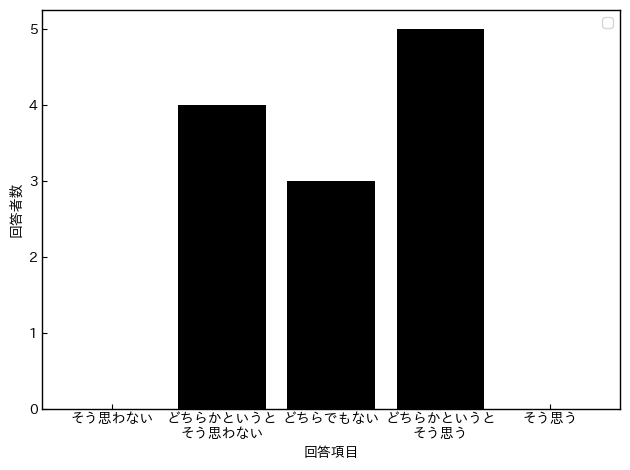
\includegraphics[height=8cm]{./fig/forecast_fukuoka_1.png}
  %\vspace{-3mm}
  \caption{(福岡)旅行中に災害に巻き込まれたとしたら、被害は大きいと思う}
  \label{fig:forecast_fukuoka_1}
  %\vspace{2mm}
\end{figure}
「そう思わない」と回答した人が0人,「どちらかというとそう思わない」と回答した人が4人,「どちらでもない」と回答した人が3人「どちらかというとそう思う」と回答した人が5人,「そう思う」と回答した人が0人いた.
災害発生の確率に対する認知への回答を図 \ref{fig:forecast_fukuoka_2}に示す.
\begin{figure}[H]
  \centering
  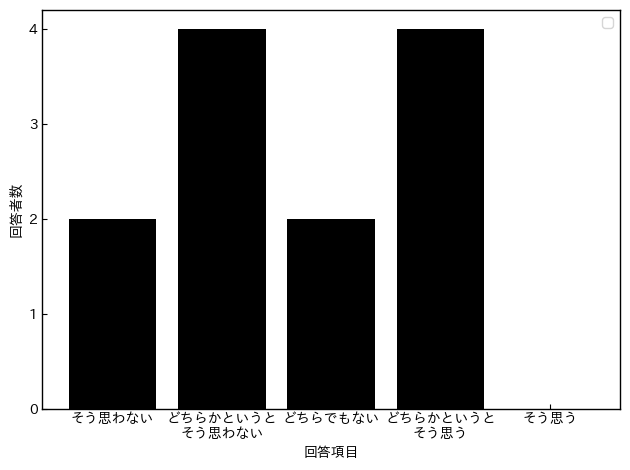
\includegraphics[height=8cm]{./fig/forecast_fukuoka_2.png}
  %\vspace{-3mm}
  \caption{(福岡)旅行中に災害の被害に遭うと思う}
  \label{fig:forecast_fukuoka_2}
  %\vspace{2mm}
\end{figure}
「そう思わない」と回答した人が2人,「どちらかというとそう思わない」と回答した人が4人,「どちらでもない」と回答した人が2人「どちらかというとそう思う」と回答した人が4人,「そう思う」と回答した人が0人いた.

\subsection{検定の結果}
得られたデータからBrunner-Munzel検定を行なった.
比較対象はシステムグループと天気予報グループの2つの旅程に対する脅威評価である.
旅程ごとに検定結果を述べる.
表に記載されている,Xは天気予報グループの標本,Yはシステムグループの標本とする.

\subsubsection{鹿児島の旅程}
鹿児島の旅程は1日先に災害の予報が出ている旅程であった.
「災害の深刻さに対する認知」と「災害発生の確率に対する認知」についての検定結果を述べる.
\par まず「災害の深刻さに対する認知」の検定結果を表 \ref{table:kagoshima_sinkoku}に示す.
P値は\quad\text{$1.504 \times 10^{-2}$}で,効果量は\quad\text{$7.5 \times 10^{-1}$}であった.

\begin{table}[h]
  \caption{1日先の旅程に対する災害の深刻さに対する認知の検定結果}
  \centering
  \begin{tabular}{|c|c|}
  \hline
  \multicolumn{1}{|c|}{p-value} &  \multicolumn{1}{c|}{\quad\text{$P(X < Y) + \frac{1}{2}P(X = Y)$}} \\
  \hline \hline
  \quad\text{$1.504 \times 10^{-2}$} & \quad\text{$7.5 \times 10^{-1}$}  \\ \hline
  \end{tabular}
  \label{table:kagoshima_sinkoku}
\end{table}

次に「災害発生の確率に対する認知」の検定結果を表 \ref{table:kagoshima_kakuritu}に示す.
P値は\quad\text{$1.423 \times 10^{-1}$}で,効果量は\quad\text{$6.791667  \times 10^{-1}$}であった.

\begin{table}[h]
  \caption{1日先の旅程に対する災害発生の確率に対する認知の検定結果}
  \centering
  \begin{tabular}{|c|c|}
  \hline
  \multicolumn{1}{|c|}{p-value} &  \multicolumn{1}{c|}{\quad\text{$P(X < Y) + \frac{1}{2}P(X = Y)$}} \\
  \hline \hline
  \quad\text{$1.423 \times 10^{-1}$} & \quad\text{$6.791667  \times 10^{-1}$}  \\ \hline
  \end{tabular}
  \label{table:kagoshima_kakuritu}
\end{table}

\subsubsection{福岡の旅程}
福岡の旅程は2日先に災害の予報が出ている旅程であった.
「災害の深刻さに対する認知」と「災害発生の確率に対する認知」についての検定結果を述べる.
\par まず「災害の深刻さに対する認知」の検定結果を表 \ref{table:fukuoka_sinkoku}に示す.
P値は\quad\text{$2.507 \times 10^{-3}$}で,効果量は\quad\text{$8.333333 \times 10^{-1}$}であった.

\begin{table}[h]
  \caption{2日先の旅程に対する災害の深刻さに対する認知の検定結果}
  \centering
  \begin{tabular}{|c|c|}
  \hline
  \multicolumn{1}{|c|}{p-value} &  \multicolumn{1}{c|}{\quad\text{$P(X < Y) + \frac{1}{2}P(X = Y)$}} \\
  \hline \hline
  \quad\text{$2.507 \times 10^{-3}$} & \quad\text{$8.333333 \times 10^{-1}$}  \\ \hline
  \end{tabular}
  \label{table:fukuoka_sinkoku}
\end{table}

次に「災害発生の確率に対する認知」の検定結果を表 \ref{table:fukuoka_kakuritu}に示す.
P値は\quad\text{$1.183 \times 10^{-1}$}で,効果量は\quad\text{$7.0  \times 10^{-1}$} であった.

\begin{table}[h]
  \caption{2日先の旅程に対する災害発生の確率に対する認知の検定結果}
  \centering
  \begin{tabular}{|c|c|}
  \hline
  \multicolumn{1}{|c|}{p-value} &  \multicolumn{1}{c|}{\quad\text{$P(X < Y) + \frac{1}{2}P(X = Y)$}} \\
  \hline \hline
  \quad\text{$1.183 \times 10^{-1}$} & \quad\text{$7.0  \times 10^{-1}$}  \\ \hline
  \end{tabular}
  \label{table:fukuoka_kakuritu}
\end{table}